\documentclass{sig-alternate-05-2015}
\graphicspath{ {./images/} }

\makeatletter
\def\@copyrightspace{\relax}
\makeatother

\begin{document}

\setcopyright{acmcopyright}

\title{Multi-Agent AI}
\subtitle{[Group Coursework 1]}

\numberofauthors{3}
\author{
\alignauthor
Aksel Cakmak\\
       \affaddr{15047472}\\
       \email{zcababc@ucl.ac.uk}
% 2nd. author
\alignauthor
Chong Yang\\
       \affaddr{18089022}\\
       \email{ucabcya@ucl.ac.uk}
% 3rd. author
\alignauthor
Chen Song \\
       \affaddr{17040773}\\
       \email{ucabcs3@ucl.ac.uk}
}

\maketitle

\section{Introduction}

Here we introduce the problem, and present the setting.

Real-time bidding (RTB) offers advertisers a way to adaptively bid for ads on a per-impression basis, in real time.
It uses data from the user's context (cookies, meta-data like the browser used, the website visited, etc..) to formulate a bid price for a certain slot.

If the auction is won, the bidder's ad is then displayed in the slot. Afterwards, the user might or might not click on the displayed ad.

RTB differs from Sponsored Search Auctions, wherein an auction mechanism tries to match advertisers that bid on certain search keywords, not on specific impressions.

Bidders have a certain budget to allocate to a certain number of bids, and (in our specific setting) want to maximise the total number of clicks they get from all the ads they display.

For a specific slot, the bidder is usually interested in some specific KPI (key performance indicator) that they use to formulate their bid (in our case, we're interested in the predicted click-through-rate of a specific slot, or pCTR).

Then, a bidder has the following dimensions to consider for its bidding campaign: \\
- How to predict the KPI (here, pCTR), the choice of a predictive model, its accuracy, etc.. \\
- How the bid is formulated wrt a given pCTR. \\

The bidder wants to optimise the number of clicks it gets by choosing a good KPI predicting model and a good bidding function (in our specific setting).
In addition to this, one other constraint there is is that the whole pipeline of KPI prediction + bid function has to be calculated with minimal latency (bids often have to be submitted within a short timeframe, like 100ms) \cite{MILLI, PHD1}.


\section{Approach and Results}

%%%%%
\subsection{Problem 1: Data Exploration and Literature Review}

\subsubsection{Literature Review}


The performance of a CTR prediction model has a direct impact on the final number of clicks generated by a campaign,
which is why a lot of work has been made on how to predict the CTR of a given slot.

Regularised Logistic Regression model have been commonly used for the task of predicting CTR \cite{LOGREG1}, but are lacking in that they require some feature engineering work and are not as accurate as newer Deep Learning based methods. \cite{DL1}

As a consequence, more Deep Learning based methods have been proposed recently, where the input features are fed into neural networks which learn the implicit nonlinear relations between the different features, and consequently report enhanced accuracies. \cite{DL2, DL3, DL5} 

Once the pipeline has a model to predict the CTR, there exist different approaches to calculating a bid wrt this pCTR.



Some very simple approaches include bidding a constant value, or choosing a random bid based on some range.
Quite naturally, these approaches don't fare as well as other more sophisticated methods, that bid a variable amount using the pCTR and the contextual information of a specific slot.  \cite{ORTB}
One more advanced approach is linear bidding: the bidding value is an affine function of the predicted CTR (pCTR).
This method fares far better than the aforementioned, but is outclassed by non-linear methods like \cite{ORTB}.

% more details on the specific models ? or leave that to the actual relevant sections ?

One challenge of this particular setting is that the bidding is budget constrained: 
the advertiser (in our setting) wants to maximize the number of clicks it gets from its impressions, for some number of slots it bids for.
Knowing how fast one should burn through the given budget is a difficult problem\cite{BID1}:
If the strategy bids relatively high values, the budget might be spent early and some potentially valuable slots might be missed.
If the strategy is relatively more conservative, then the budget might not be fully spent and some valuable slots might be underbid on.
The problem is even more complex when considering the fact that there are a number of heterogeneous and unpredictable other agents with their own bidding strategies competing against a given bidder. \cite{BID1}
Determining the best rate of spending is an open question. \cite{OPENQ}



\subsubsection{Data Exploration}

We analysed some aspects of the data with respect to the weekdays, the CPC, CTR, and payprice.

\begin{figure}
\centering
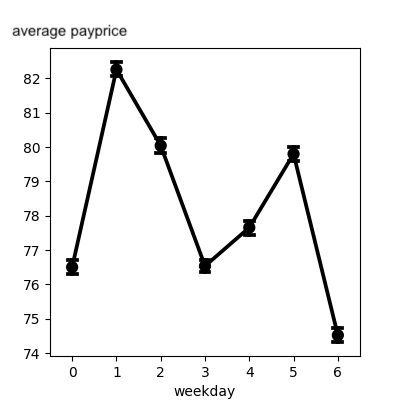
\includegraphics[height=2in, width=2in]{images/weekday_AC.png}
\caption{Average Payprice wrt Weekday}
\end{figure}

\begin{figure}
\centering
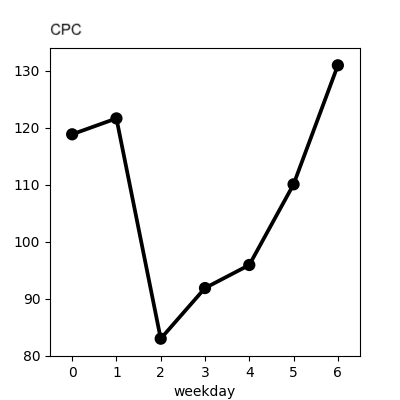
\includegraphics[height=2in, width=2in]{images/weekday_CPC.png}
\caption{Average CPC wrt Weekday}
\end{figure}

\begin{figure}
\centering
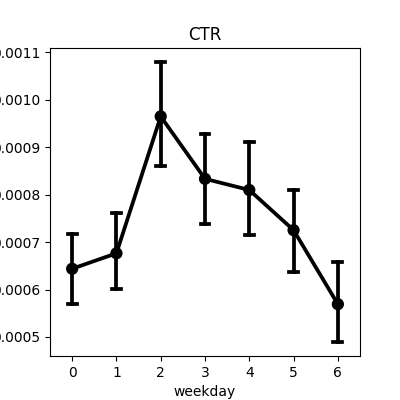
\includegraphics[height=2in, width=2in]{images/weekday_CTR.png}
\caption{Average CTR wrt Weekday}
\end{figure}

As one can see on the figures below, CPC, CTR, and payprice are extremely variable throughout the week.
The day with the lowest average CPC of 81 is day 2, and the highest CPC of 130 is attained on day 6.
The CTR per weekday falls within the range of 0.0006 (at day 6) and 0.00095 at day 2.
Finally, the payprice per weekday also belongs to a notable range, from 74 (on day 6) to 82 (on day 1).

From further analysis, we observed that the CTR per slot and payprice per slot are positively correlated;
This makes sense for our setting: assuming reasonable KPI predictive models, a slot with a high CTR would also tend to have a high pCTR,
meaning it would also have a higher private value to bidders, and from this a higher payprice from the higher bids.





%%%%
\subsection{Problem 2: Basic Bidding Strategy}
In this section, we analyse two basic bidding strategies, which are Constant Bidding Strategy and Random Bidding Strategy, and evaluate their performance based on the number of clicks within a limited budget of 6,250 CNY fen. 
Evaluation function: For the single-agent basic bidding strategies, the main metric to rank the strategies are based on the clicks from winning impressions.

\subsubsection{Constant Bidding Strategy}
In order to find an optimal constant value, we loop the constant bid prices from 0 to 300, which are the minimum bid price and maximum bid price, to find out the bid price with the highest clicks from winning impressions. Specifically, for each constant price, we retrieve the columns of 'payprice' and 'click' for all the bids in the training set. Then we compare our constant bid price with the 'payprice' for each bid and add up the click into our total clicks if our constant bid price is great than or equal to the 'payprice' while the total spend is calculated at the mean time. Afterwards we remove the clicks from bottom to top where the total spend has been over our limited budget.
In order to use the training set to find out a good price for validation set, initially we need to normalize the budget based on equation 1.

\begin{equation}budget_{train}=\frac{sizeOfTrain}{sizeOfValidation} * budget_{validation}\end{equation}

Analysis: 
Figure 1 shows that how the value of click changes based on the increment of the constant bidding price. The clicks increase dramatically when the constant bidding price increases from 1 to 78 and the climax of clicks is 643 when the constant bidding price is 77. Then the clicks drop smoothly when the bidding price increases from 78 to 300.


Figure 2 shows the changes of click value depending on bid price in the validation set with the standard budget. We could see the clicks are relatively high when the bid price is between 70 to 100. Surprisingly, the value of click is maximised as 68 when the bidding price is 77 or 79. Therefore, the finding in our training data is perfectly match the validation set.

\begin{figure}
\centering
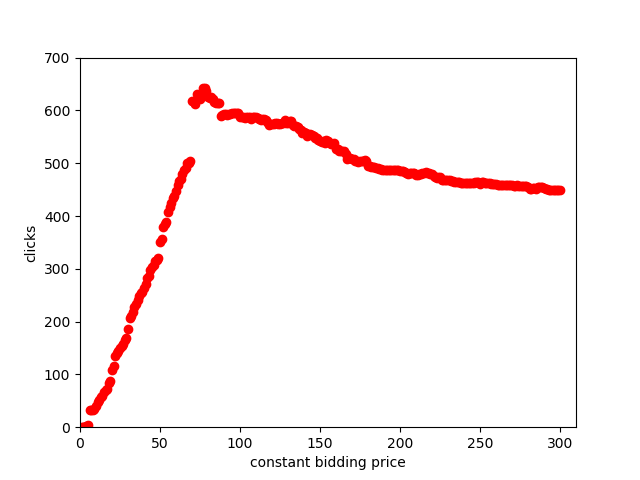
\includegraphics[height=2in, width=2in]{images/constant_bidding.png}
\caption{Training set - bid price and clicks}
\end{figure}

\begin{figure}
\centering
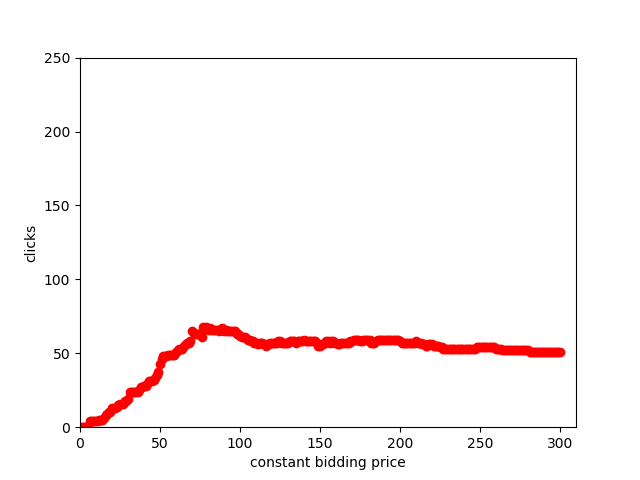
\includegraphics[height=2in, width=2in]{images/constant_bidding_validation.png}
\caption{Validation set - bid price and clicks}
\end{figure}




\subsubsection{Random Bidding Strategy}
In order to find the optimal bidding range for random bidding, we step through a range of lower bound and a range of upper bound to find out the bid price with the highest clicks from winning impressions. Similarly, we use the same method as the one in Constant Bidding Strategy to calculate the clicks. 

Analysis: 
The highest clicks are 628 generated from range 10 to 130 in the training set with the limited normalised budget. In the validation set, we find the highest clicks are 76 generated from the range 20 to 150. It is acceptable that the best range in these two sets are not far from each other.


\subsubsection{Competition among homogeneous random bidding agents}

Competition among homogeneous random bidding agents:
In the sub-problem, we first step into different combinations of lower bound and upper bound. And for each pair of lower bound and upper bound, we generate n agents who are using random bidding strategy with the price with the selected bounds. Then we add the click to the winner following criterion 2 for each bid. 
Our criterion for bound comparison: the average click among the agents is criterion of winning bounds. And the optimal bounds should generate the highest average clicks (total clicks). Table 2 is  optimal bounds and total clicks of different number of agents. 


\begin{table}
\centering
\caption{Optimal Bounds and Clicks}
\begin{tabular}{|c|c|c|c|c|c|l|} \hline
agent number&50&60&70&80&90&100\\ \hline
lower bound&90&90&110&70&130&50\\ \hline
upper bound&300&300&300&300&300&300\\ \hline
clicks&202& 202&202&202&202&202\\
\hline\end{tabular}
\end{table}

Consequently, the optimal upper bound is 300 for all of the group of multiple agent bidding, which is much higher than the single agent bidding. The reason for this high upper bound is that the strategy of multiple agent bidding is to maximize the total number of clicks, and the higher upper bound is, the larger opportunity that the total clicks could be maximised. In other words, the strategy for multi-agent random bidding to is maximize the benefits of the group.

%%%%%
\subsection{Problem 3: Linear Bidding Strategy}
In order to apply CTR estimation to for a linear bidding strategy, we initially retrieve the these features as independent variables X: day, hour, region, ad exchange, slot width, slot height, advertiser, slot visibility, slot format, OS, browser, and slot price from the data set. Specifically, we categorise the slot price to five categories based on the price values, and we extract the OS and browser from the column useragent. And the rest features could be simply fetched from the data. The click from the data is our predictor Y.
Afterwards, we import the Logistic Regression model from sklearn and train the model with the independent variables and predictor from the training set. Then we use the trained model to predict the click of test data and validation data separately. The pCTR of the validation data could be calculated with the equation 2.
\begin{equation}pCTR=\frac{numOfClicks}{numOfWinningImpressions}\end{equation}

The bid price for each bid is calculated as equation 3. As shown in Figure 3, the total clicks increase sharply when base bid increases from 1 to 20 and drop smoothly after then. The value clicks is maximised as 39 when the base bid is 20.

\begin{equation}bidPrice=\frac{baseBidPrice*pCTR}{avgCTR}\end{equation}

\begin{figure}
\centering
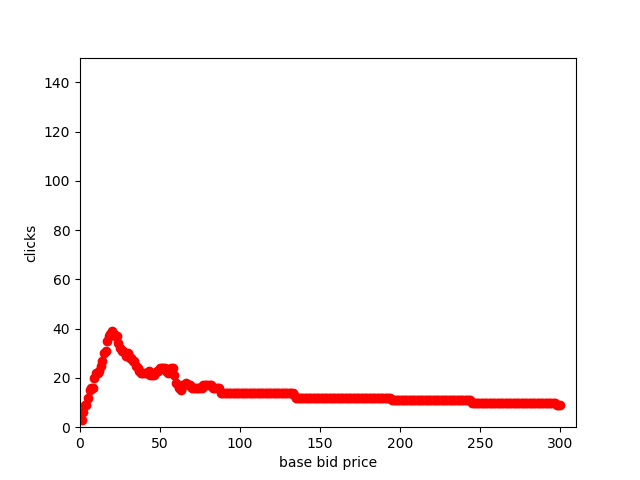
\includegraphics[height=2in, width=2in]{images/base_bid_price.png}
\caption{Validation set - base price and clicks}
\end{figure}

Comparison:
\begin{table}
\centering
\caption{Behaviour Comparison}
\begin{tabular}{|c|c|c|l|} \hline
&Constant Bidding&Random Bidding&Linear Bidding\\ \hline
price&79&range(20, 150)&67(base)\\ \hline
clicks&68& 76&124\\
\hline\end{tabular}
\end{table}

Obviously, the behaviour of the linear bidding strategy is much better than random bidding and constant bidding strategies. The optimal value of clicks in linear bidding is 124 while the ones of constant bidding and random bidding are merely 68 and 76 separately.

%%%%%%%
\subsection{Problem 4: Non-Linear Bidding Strategy}
We calculate the non-linear bidding price based on ORTB (equation 4), and we step through some combination of c and lambda to find the optimal pair generating the optimal bid prices. We find the value of clicks is 39 when c equals to 39 and lambda equals to 1.31072e-05. Therefore, our non-linear bidding strategy just generates the same result as linear bidding strategy.
\begin{equation}bidPrice=\sqrt{\frac{c}{\lambda} * pCTR + c^2} - c\end{equation}


%%%%%%%
\subsection{Problem 5: Multi-agent Bidding Strategy}

In order to find a good bid strategy for Winning criterion 2, we train a multi-agent model where 80 agents attend to the competition by using different strategies:

1)	There are 20 agents using constant bidding strategies with constant bidding prices from 110 to 300 intervals 10.

2)	There are 20 agents using the same random bidding strategy found in previous sub-problem 2.2.3 (multi-agent random bidding strategy).

3)	There are 20 agents using linear bidding strategies with the base bid prices from 110 to 300 intervals 10.

4)	In order to find a good strategy for non-linear bidding, we run a twenty-agent competition with different combination of parameters (c and lambda are equal to 50 and 2.048e-07 separately) to find the optimal non-linear strategy. Then there are 20 agents using this same non-linear bidding strategy.

Then we concatenate the bid prices of these 80 agents together, assign each agent limited budget, and start the competition. The agent wins in a bid if his or her bid in this row is greater than or equal to all the other agents as well as the pay price in the data. And this agent could gain a click if there is a click in this winning bid. Moreover, this agent needs to pay the second highest price and his budget will decrease by that price. Table 3 show the agent with the highest number of clicks in each strategy.

\begin{table}
\centering
\caption{Best performance}
\begin{tabular}{|c|c|c|c|l|} \hline
&Constant &Random &Linear&Non-linear\\ \hline
highest click&3&2&20&12\\
\hline\end{tabular}
\end{table}

Analysis:

1)	As expectation, both constant bidders and random bidders have a poor performance in this competition since they do not adjust their price based on data strategically.

2)	Surprisingly, the best performer among the linear bidders gain a higher clicks than the best performer among the non-linear bidders. In our opinions, the reason for this behaviour is that we did not implement enough training on the parameter discovery. Ideally, we are supposed to attempt more combination of parameters and implement the competition with more agents instead of merely twenty agents.

\section{Conclusion}

We recap on what we did for each problem.

We started off by building a simple agent that bid a constant value for all slots, then found the optimal value of the bid to maximize the number of clicks earned by our agent.
Then we built a bidder that chose a random bid from within a certain range for each slot, and found an optimal range.
We then modelled 50-100 of these agents and studied the performance of the random bidding model in this setting.
For the next part, we used a Logistic Regression model to predict the CTR of ad slots, and bid an amount linearly proportional to the predicted CTR.
Then, keeping our predictions from the previous part, we built a non-linear bidding function.
Finally, we simulated a number of heterogeneous agents to compete for the slots and analysed our model's performance in this setting.

%
%When we compare these four strategies for a single agent bidding, the performance rankings from high to low are Non-linear bidding strategy, Linear bidding strategy, random bidding strategy, and constant bidding strategy. 
%However, surprisingly, in our multiply agent competition, the Linear bidding strategy performs better than Non-linear bidding strategy. 
%We conclude that this phenomenon is because of the lack of training in the optimal parameter exploration for Non-linear bidding. It averagely takes four hours for a competition of twenty agents non-linear bidding with five hundred combination of parameter c and lambda. In order to improve our multiply agent non-linear bidding strategy, more combination should be evaluated.








%
%\subsection{Citations}
%Citations to articles \cite{bowman:reasoning,
%clark:pct, braams:babel, herlihy:methodology},
%conference proceedings \cite{clark:pct} or
%books \cite{salas:calculus, Lamport:LaTeX}




%\bibliographystyle{abbrv}
%\bibliography{sigproc}
\begin{thebibliography}{9}

\bibitem{LOGREG1} 
H. Brendan Mcmahan, H. Brendan Holt, et al. 2014. 
Ad Click Prediction: a View from the Trenches. 
In Proceedings of the 19th ACM SIGKDD International Conference on Knowledge Discovery and Data Mining. 1222-1230.

\bibitem{PHD1} 
Weinan Zhang et al. 2014.
Optimal real-time bidding for display advertising.
Proceedings of the 20th ACM SIGKDD international conference on Knowledge discovery and data mining.

\bibitem{DL1} 
Guorui Zhou et al. 
Deep Interest Network for Click-Through Rate Prediction.
In Proceedings of the 24th ACM SIGKDD International Conference on Knowledge Discovery \& Data Mining.

\bibitem{DL2}
Paul Covington, Jay Adams, and Emre Sargin. 2016. 
Deep neural networks for youtube recommendations. 
In Proceedings of the 10th ACM Conference on Recommender Systems. ACM, 191-198.

\bibitem{DL3}
Cheng H. et al. 2016. Wide \& deep learning for recommender systems. 
In Proceedings of the 1st Workshop on Deep Learning for Recommender Systems. ACM.

\bibitem{DL4}
Ying Shan, T Ryan Hoens, Jian Jiao, Haijing Wang, Dong Yu, and JC Mao. Deep
Crossing: Web-scale modeling without manually crafted combinatorial features.

\bibitem{DL5}
Shuangfei Zhai, Keng-hao Chang, Ruofei Zhang, and Zhongfei Mark Zhang. 2016.
Deepintent: Learning attentions for online advertising with recurrent neural networks. 
In Proceedings of the 22nd ACM SIGKDD International Conference on Knowledge Discovery and Data Mining. ACM, 1295-1304.

\bibitem{MILLI}
Shuai Yuan, Jun Wang, and Xiaoxue Zhao. Real-time bidding for online advertising: measurement and analysis. 
In Proceedings of the Seventh International Workshop on Data Mining for Online Advertising, page 3. ACM, 2013.

\bibitem{ORTB}
Weinan Zhang, Shuai Yuan, and Jun Wang. Optimal real-time bidding for display advertising. 
In Proceedings of the 20th ACM SIGKDD international conference on Knowledge discovery and data mining, pages 1077-1086. ACM, 2014.

\bibitem{BID1}
Di Wu et al.
Budget Constrained Bidding by Model-free Reinforcement Learning in Display Advertising. ACM, 2018.

\bibitem{OPENQ}
Yunhong Zhou, Deeparnab Chakrabarty, and Rajan Lukose. 2008. 
Budget constrained bidding in keyword auctions and online knapsack problems. 
In International Workshop on Internet and Network Economics. Springer, 566-576.

\end{thebibliography}


\end{document}






